\documentclass{article}
\usepackage{amsmath}
\usepackage{amssymb}
\usepackage{graphicx}
\usepackage{amsthm}
\usepackage{empheq}
\usepackage{float}
\usepackage[utf8]{inputenc}
\usepackage{amssymb}
\usepackage[most]{tcolorbox}
\usepackage{hyperref}

\newtheorem*{theorem}{Thm}
\newtheorem*{proposition}{Prop}
\theoremstyle{definition}
\newtheorem*{definition}{Defn}

\theoremstyle{remark}
\newtheorem*{remark}{Remark}

\theoremstyle{example}
\newtheorem*{example}{Ex}

\newtcbox{\mymath}[1][]{%
    nobeforeafter, math upper, tcbox raise base,
    enhanced, colframe=blue!30!black,
    colback=blue!30, boxrule=1pt,
    #1}
\title{Solution to coupled linear oscillator}

\begin{document}

\maketitle

\section*{Coupled linear oscillators revisited}
Let us consider again the chain of coupled oscillators with Lagrangian
$$
L = \frac{1}{2}\sum_i^N \dot x_i^2 m_i - \frac{1}{2}\sum_{i,j, |i-j|=1}^N k_{i}(x_i-x_j)^2.
$$
The constrained sum in the potential asserts that only nearest neighbors. We saw that the equations of motion can be written in matrix form:
$$
(\mathbf M \partial_t^2-\mathbf K )\vec x(t) = 0
$$
We can render this EOM algebraic by a Fourier transform:
$$(\mathbf M \omega^2+\mathbf K )\vec x(\omega) = 0.
$$
Let's take a more direct approach than last time and try to obtain the modes of oscillation and the trajectories. First, notice that any physically meaningful mass matrix must be invertible (it is always diagonal and positive, actually). Then,
\begin{align*}
  \mathbf{M}^{-1}(\mathbf M \omega^2+\mathbf K) \vec x(\omega)&=\mathbf{M}^{-1}0 \\
  (\mathbb I \omega^2+\underbrace{\mathbf{M}^{-1}\mathbf K}_{\bar {\mathbf K}})\vec x(\omega)&=0\\
  \bar{\mathbf K}\vec x(\omega) = -\omega^2 \vec x(\omega)
\end{align*}
We have therefore formulated the EOM as an eigenvalue equation: $-\omega^2$ is the eigenvalue of eigenvector $\vec x(\omega)$. For small matrices, the eigenvalues can be computed by hand using
$$
\det(\omega^2\mathbb I - \bar{\mathbf K})=0 \text{ (look familiar?)}.
$$
This will yield a set of eigenvalues, $\{\omega_i\}$ which are, in general, complex \begin{footnote}{\emph{All} square matrices over $\mathbb C$ have (complex) eigenvalues. The same is not true for the reals (because $\mathbb R$ is not algebraically closed)}\end{footnote}. We then plug this back into the equation and solve for the $i$-th eigenvector: $\bar{\mathbf K }\vec x_i(\omega_i)=-\omega_i^2x_i(\omega_i)$. Of course, in real life such things are never computed by hand. One would either diagonalize numerically or use some form of symbolic math software like Mathematica or Sage. 

We will walk through a specific computation in class where you will get to practice this technique. 

\section*{The double pendulum}

The double pendulum is an important example so let's go through the construction of its Lagrangian.

\begin{figure}[H]
  \centering
  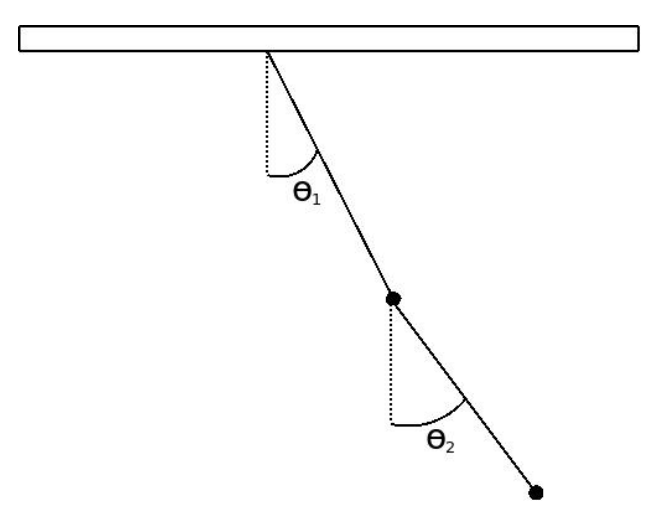
\includegraphics[width=0.5\textwidth]{Capture.PNG}
\end{figure}
We have two generalized coordinates, $\theta_1,\theta_2$ which relate to the Cartesion coordinates as
\begin{align*}
  q_1 &= (L_1\sin\theta_1,-L_1\cos \theta_1)\\
  q_2 &= q_1+(L_2\sin\theta_1, -L_2\cos\theta_2)
\end{align*}
We can then construct the Lagrangian as 
$$
\mathcal L=\frac{1}{2}m_1L_1^2\dot\theta_i^2+\frac{1}{2}m_2L_1^2\dot\theta_1^2+\frac{1}{2}m_2L_2^2\dot\theta^2_2+m_1gL_1\cos\theta_1+m_2(L_1\cos\theta_1+L_2\cos\theta_2)
$$
You can, and should, show that the EOM is given by the matrix equation
$$
(\mathbf M\partial^2_t+\mathbf K)\vec\theta=0
$$
with $\mathbf M$ and $\mathbf K$ suitably defined. If $m_1=m_2$ and $L_1=L_2$, you obtain what is given to you in the problem sheet. 

\href{https://matplotlib.org/stable/gallery/animation/double_pendulum.html}{Here} is a numerical implementation in python. They use odeint to integrate the EOM directly. You'll notice that they hard code the number of degrees of freedom. If instead of odeint you numerically compute the eigenvectors and eigenvalues of $\mathbf M^{-1}\mathbf K$ (then inverse Foureri transform), you can generalize to the $N$-pendulum problem.   



\end{document}

\begin{empheq}[box=\tcbhighmath]{align*}
    F_r&=m(\ddot r-r\dot \theta^2-r\dot\phi^2\sin^2\theta)\\
  F_\theta&=m(2\dot r\dot \theta+r\ddot \theta-r\dot\phi^2\sin\theta\cos\theta)\\
  F_\phi&=m(r\ddot \phi \sin \theta +2\dot r \dot \phi \sin \theta +2r\dot\theta \dot \phi\cos\theta)
\end{empheq}
